\documentclass[border=2pt]{standalone}
\usepackage{pgfplots}
\usepackage{tikz}
\usetikzlibrary{arrows}
\usetikzlibrary{patterns}

\definecolor{v0}{HTML}{1b7837}
\definecolor{v1}{HTML}{7fbf7b}
\definecolor{v2}{HTML}{a6611a}
\definecolor{v3}{HTML}{a6cee3}

%\definecolor{v0}{HTML}{018571}
%\definecolor{v1}{HTML}{80cdc1}
%\definecolor{v2}{HTML}{a6611a}
%\definecolor{v3}{HTML}{dfc27d}

\begin{document}

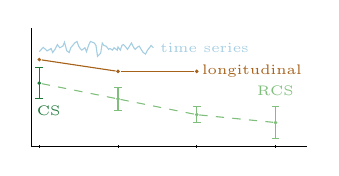
\begin{tikzpicture}[scale=1.0]

%\draw[] (0.9,0.3) -- (0.9, 1.8);
%\draw[] (0.8,0.4) -- (4.3, 0.4);

\draw[line width=0.1mm] (0.9,0.4) -- (0.9, 1.9);
\draw[line width=0.1mm] (0.9,0.4) -- (4.4, 0.4);
%\draw[line width=0.1mm] (0.8,1.9) -- (4.4, 1.9);
%\draw[line width=0.1mm] (4.4,0.4) -- (4.4, 1.9);

\draw[line width=0.1mm] (1,0.38) -- (1,0.42);
\draw[line width=0.1mm] (2,0.38) -- (2,0.42);
\draw[line width=0.1mm] (3,0.38) -- (3,0.42);
\draw[line width=0.1mm] (4,0.38) -- (4,0.42);

\draw[color=v0] (1,1.2) node[circle,fill,inner sep=0.5pt](d1){};
\draw[color=v0] (1,1) -- (1,1.4);
\draw[color=v0] (0.95,1) -- (1.05,1);
\draw[color=v0] (0.95,1.4) -- (1.05,1.4);

\draw[color=v1] (2,1.0) node[circle,fill,inner sep=0.5pt](d2){};
\draw[color=v1] (2,0.85) -- (2,1.15);
\draw[color=v1] (1.95,0.85) -- (2.05,0.85);
\draw[color=v1] (1.95,1.15) -- (2.05,1.15);

\draw[color=v1] (3,0.8) node[circle,fill,inner sep=0.5pt](d3){};
\draw[color=v1] (3,0.70) -- (3,0.90);
\draw[color=v1] (2.95,0.70) -- (3.05,0.70);
\draw[color=v1] (2.95,0.90) -- (3.05,0.90);

\draw[color=v1] (4,0.7) node[circle,fill,inner sep=0.5pt](d4){};
\draw[color=v1] (4,0.5) -- (4,0.90);
\draw[color=v1] (3.95,0.5) -- (4.05,0.5);
\draw[color=v1] (3.95,0.90) -- (4.05,0.90);

\draw[color=v1,dashed] (d1) -- (d2);
\draw[color=v1,dashed] (d2) -- (d3);
\draw[color=v1,dashed] (d3) -- (d4);

\draw[color=v2] (1,1.5) node[circle,fill,inner sep = 0.5pt](l1){};
\draw[color=v2] (2,1.35) node[circle,fill,inner sep = 0.5pt](l2){};
\draw[color=v2] (3,1.35) node[circle,fill,inner sep = 0.5pt](l3){};

\draw[color=v2] (l1) -- (l2);
\draw[color=v2] (l2) -- (l3);

\draw[color=v3] (1,1.6) -- (1.05,1.655) -- (1.1,1.61) -- (1.15,1.64) -- (1.17,1.59) -- (1.2,1.63) -- (1.23,1.69) -- (1.26,1.65) -- (1.30,1.67) -- (1.32,1.72) -- (1.35,1.61) -- (1.38,1.59) -- (1.40,1.65) -- (1.45,1.71) -- (1.48,1.73) -- (1.50,1.67) -- (1.52,1.64) -- (1.54,1.62) -- (1.58,1.65) -- (1.60,1.60) -- (1.63,1.69) -- (1.65,1.73) -- (1.70,1.71) -- (1.72,1.68) -- (1.74,1.54) -- (1.78,1.58) -- (1.80,1.71) -- (1.82,1.68) -- (1.85,1.67) -- (1.88,1.63) -- (1.90,1.64) -- (1.93,1.62) -- (1.95,1.65) -- (1.99,1.62) -- (2, 1.66) -- (2.03,1.62) -- (2.05,1.68) -- (2.07,1.69) -- (2.09,1.67) -- (2.12,1.63) -- (2.14,1.66) -- (2.17, 1.71) -- (2.20, 1.65) -- (2.22, 1.63) -- (2.25,1.66) -- (2.27,1.67) -- (2.30,1.62) -- (2.32,1.59) -- (2.35, 1.57) -- (2.37,1.61) -- (2.39,1.64) -- (2.40, 1.65) -- (2.42, 1.68) -- (2.45,1.65);

\node[text=v3] at (3.1,1.65){\tiny time series};
\node[text=v2] at (3.7,1.35){\tiny longitudinal};
\node[text=v1] at (4.0,1.1){\tiny RCS};
\node[text=v0] at (1.12,0.85){\tiny CS};

\end{tikzpicture}





\end{document}
